%\documentclass[11pt,twocolumn,twoside]{IEEEtran}
%\usepackage{amsmath}
%\usepackage[pdftex]{epsfig}
%\usepackage{amsfonts}
%\usepackage{amssymb}
%\usepackage{fancyhdr}
%\usepackage{mycommands,url,cite,hyperref,caption,subfigure}
%\include{graphicsx}

%\pagestyle{fancy}
%%\renewcommand{\headrulewidth}{0pt}
%\renewcommand{\footrulewidth}{0pt}
%\rhead{\includegraphics[height=0.6in]{CITransparentwithTitleForWeb.png}}
%\fancyhead[LO]{\sc Selecting Predictors of Indian Monsoon} % shorter form of title to fit in space
%\fancyhead[LE]{\sc Majumdar, Dietz, Chatterjee} % author list or et al., to fit in space
%\chead{}
%\cfoot{}

%\begin{document}
%\title{\vspace{0.2in}\sc Identifying Driving Factors Behind Indian Monsoon Precipitation using Model Selection based on Data Depth}
%\author{Subhabrata Majumdar$^1$\thanks{Corresponding author: S. Majumdar, University of Minnesota Twin Cities, Minneapolis MN; majum010@umn.edu$^1$}, Lindsey Dietz$^1$, Snigdhansu Chatterjee$^1$}
%
%\maketitle
%\thispagestyle{fancy}

%\begin{abstract}
%We introduce a novel one-step model selection technique for general regression estimators, and implement it in a linear mixed model setup to identify important predictors affecting Indian Monsoon precipitation. Under very general assumptions, this technique correctly identifies the set of non-zero values in the true coefficient (of length $p$) by comparing only $p+1$ models. Here we use wild bootstrap to estimate the selection criterion. Mixed models built on predictors selected by our procedure are more stable and accurate than full models across testing years in predicting median daily rainfall at a station.
%\end{abstract}

\section{Identifying Driving Factors Behind Indian Monsoon Precipitation}
\label{Section:IndianMonsoon}
%
Various  studies indicate that our knowledge about the physical drivers of precipitation in India is incomplete; this is in addition to the known difficulties in modeling precipitation itself \citep{KnuttiEtal10, TrenberthEtal03, WangEtal05, Trenberth11}. For example, \cite{Goswami05} discovered an upward trend in frequency and magnitude of extreme rain events, using daily central Indian rainfall data on a $10^{\circ}$ $\times$ $12^{\circ}$ grid, but a similar study on a $1^{\circ}\times 1^{\circ}$ gridded data by \cite{GhoshEtal16} suggested that there are both increasing and decreasing trends of extreme rainfall events, depending on the location. Additionally, \cite{Krishnamurthy09} reported increasing trends in exceedances of the 99th percentile of daily rainfall; however, there is also a decreasing trend for exceedances of the 90th percentile data in many parts of India. Significant spatial and temporal variabilities at various scales have also been discovered for Indian Monsoon \citep{Dietz2014, Dietz2015Chapter}.

Here we attempt to identify the driving factors behind precipitation during the Indian monsoon season using our $e$-value based model selection technique. Data is obtained from the repositories of the National Climatic Data Center (NCDC) and National Oceanic and Atmospheric Administration (NOAA), for the years 1978-2012. 
We obtained data 35 potential covariates of the Indian summer precipitation:

\noindent\textbf{(A) Station-specific}: (from 36 weather stations across India) Latitude, longitude, elevation, maximum and minimum temperature, tropospheric temperature difference ($\Delta TT$), Indian Dipole Mode Index (DMI), Ni\~{n}o 3.4 anomaly;

\noindent\textbf{(B) Global}:
\begin{itemize}
\item $u$-wind and $v$-wind at 200, 600 and 850 mb;

\item 10 indices of Madden-Julian Oscillations: 20E, 70E, 80E, 100E, 120E, 140E, 160E, 120W, 40W, 10W;

\item Teleconnections: North Atlantic Oscillation (NAO), East Atlantic (EA), West Pacific (WP), East Pacific-North Pacific (EPNP), Pacific/North American (PNA), East Atlantic/Western Russia (EAWR), Scandinavia (SCA), Tropical/Northern Hemisphere (TNH), Polar/Eurasia (POL);

\item Solar Flux;

\item Land-Ocean Temperature Anomaly (TA).
\end{itemize}

These covariates are all based on existing knowledge and conjectures from the actual Physics driving Indian summer precipitations. The references provided earlier in this section, and multiple references contained therein may be used for background knowledge on the physical processes related to Indian monsoon rainfall, which after decades of study remains one of the most challenging problems in climate science.

\begin{table}
\centering
\begin{scriptsize}
   \begin{tabular}{l|l}
    \hline
      Variable dropped      & $\hat e_n (\cS_{-j})$        \\ \hline
    - Tmax                  & 0.1490772 \\
    - X120W                 & 0.2190159 \\
    - ELEVATION             & 0.2288938 \\
    - X120E                 & 0.2290021 \\
    - $\Delta TT$\_Deg\_Celsius & 0.2371846 \\
    - X80E                  & 0.2449195 \\
    - LATITUDE              & 0.2468698 \\
    - TNH                   & 0.2538924 \\
    - Nino34                & 0.2541503 \\
    - X10W                  & 0.2558397 \\
    - LONGITUDE             & 0.2563105 \\
    - X100E                 & 0.2565388 \\
    - EAWR                  & 0.2565687 \\
    - X70E                  & 0.2596766 \\
    - $v$\_wind\_850          & 0.2604214 \\
    - X140E                 & 0.2609039 \\
    - X40W                  & 0.261159  \\
    - SolarFlux             & 0.2624313 \\
    - X160E                 & 0.2626321 \\
    - EPNP                  & 0.2630901 \\
    - TempAnomaly           & 0.2633658 \\
    - u\_wind\_850          & 0.2649837 \\
    - WP                    & 0.2660394 \\ \hline
    $<$none$>$                  & 0.2663496 \\ \hline
    - POL                   & 0.2677756 \\
    - Tmin                  & 0.268231  \\
    - X20E                  & 0.2687891 \\
    - EA                    & 0.2690791 \\
    - $u$\_wind\_200          & 0.2692731 \\
    - $u$\_wind\_600          & 0.2695297 \\
    - SCA                   & 0.2700276 \\
    - DMI                   & 0.2700579 \\
    - PNA                   & 0.2715089 \\
    - $v$\_wind\_200          & 0.2731708 \\
    - $v$\_wind\_600          & 0.2748239 \\
    - NAO                   & 0.2764488 \\ \hline
    \end{tabular}
\end{scriptsize}
\caption{Ordered values of  $\hat e_n (\cS_{-j})$ after dropping the $j$-th variable from the full model in the Indian summer precipitation data}
\label{table:raintable}
\end{table}

\begin{figure}
\begin{center}

\begin{tabular}{cc}
		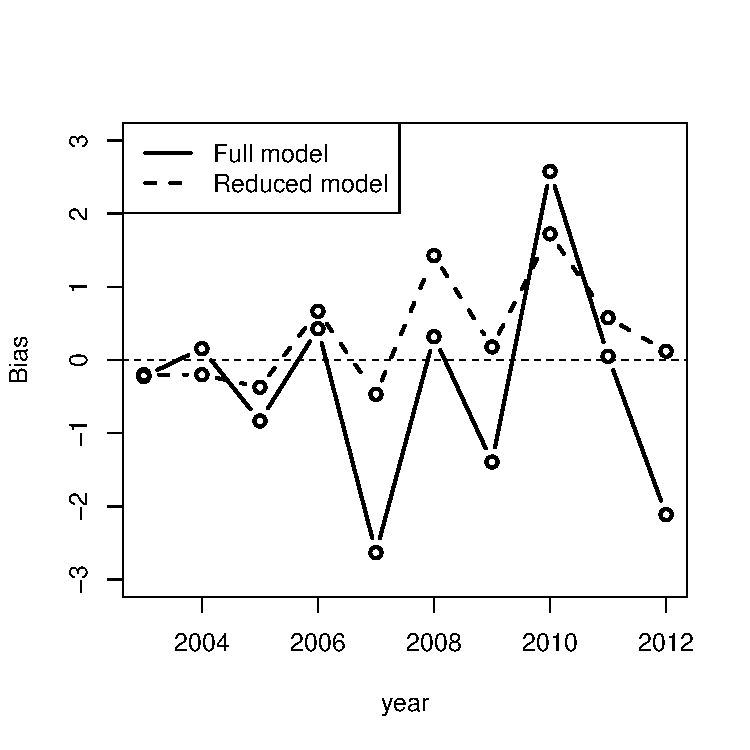
\includegraphics[width=0.32\textwidth]{Chapter-appli/rolling_predbias_full_vs_reduced_gamma.pdf}
	& 
		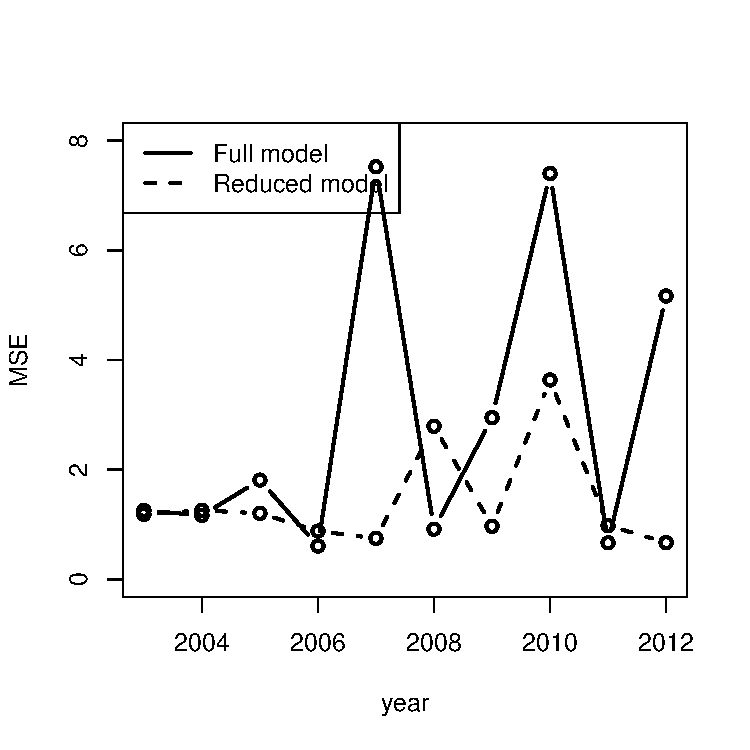
\includegraphics[width=0.32\textwidth]{Chapter-appli/rolling_predMSE_full_vs_reduced_gamma.pdf} \\
	(a) & (b) \\	
		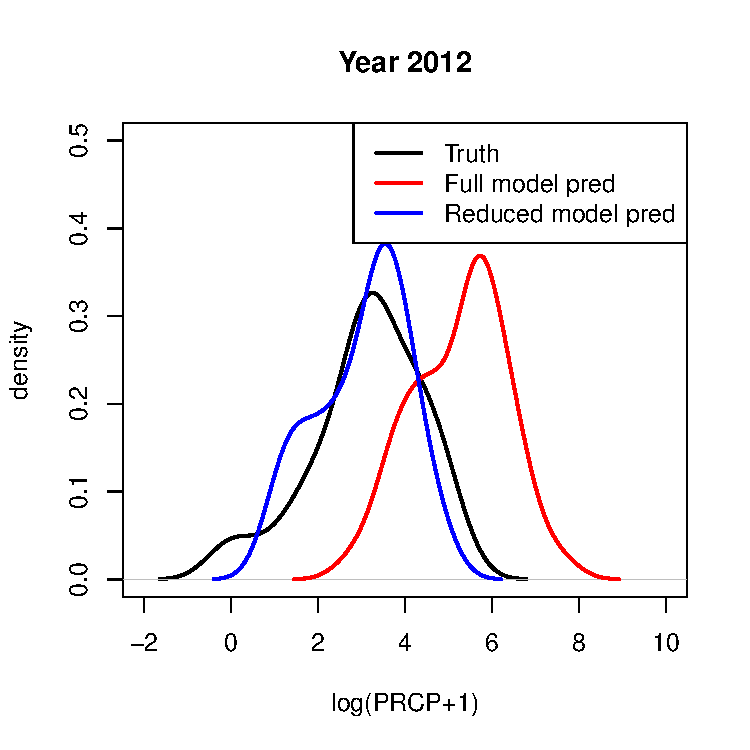
\includegraphics[width=0.32\textwidth]{Chapter-appli/rolling_density2012_full_vs_reduced_gamma.pdf}
	& 
		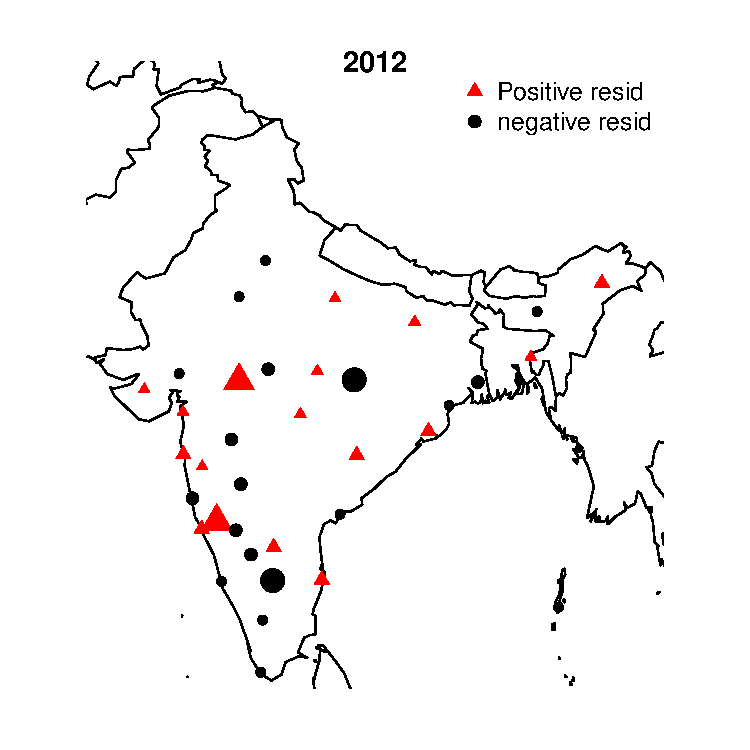
\includegraphics[width=0.32\textwidth]{Chapter-appli/rolling_map2012_full_vs_reduced_gamma.pdf} \\
	(c) & (d) \\	
\end{tabular}

\caption{Comparing full model rolling predictions with reduced models: (a) Bias across years, (b) MSE across years, (c) density plots for 2012, (d) stationwise residuals for 2012}
\label{fig:prepost}

\end{center}
\end{figure}

As a modeling step, we consider the  annual medians of all the above covariates as fixed effects, the log yearly rainfall at a weather station as response variable, and include year-specific random intercepts. \ref{table:raintable} lists the estimated $\hat{e} (\cS_{ -j})$ values in increasing order for the full model as well as all 35  models where a single variable is dropped. We implement the gamma bootstrap with Monte Carlo resample sizes $R = R_1 = 1000$. We use data until 2002 as training data, which contains $n=897$ samples. The mixed effects model trained on this data is evaluated for $\tau_n = n^\gamma; \gamma = 0.01, 0.02, \ldots, 0.16$. We take the covariate set corresponding to the tuning parameter which minimizes future fixed effect prediction errors on the testing data, i.e. for the period 2003-2012. Outputs of the fast $e$-value procedure for this covariate set are listed in \ref{table:raintable}. The variables listed above {\textit{none}} in this table are considered relevant by our $e$-value criterion.

All the variables selected by our procedure have documented effects on Indian monsoon \citep{KrishChapter, MoonWangHa12}. The single largest contributor is {\textit{maximum temperature}}, whose relation to  precipitation is based on the Clausius-Clapeyron relation is now classical knowledge in Physics. It seems 
that wind velocities high up in the atmosphere are not significant contributors, and the fact that many covariates are selected in the process highlights the complexity of the system.

%TA seems to have a large influence. Several MJO indices are selected when starting from a 
%full model with everything but TA, but are dropped in favor of TA when it is included in 
%the full model. The EPNP and the 120E index of MJO quantify intraseasonal oscillations in 
%sea-surfact temperature and troposhperic air circulation, respectively, and in our 
%analysis both get selected with very close values of $C_n$.

To check out-of-sample prediction performance of the estimated minimal adequate, we use a rolling validation scheme. For each of the 10 test years: 2003--2012, we select important variables from the model built on past 25 year's data (i.e. use data from 1978--2002 for 2003, 1979-2003 for 2004 and so on), build a model using them and compare predictions on test year obtained from this model with those from the full model. \ref{fig:prepost} summarizes results obtained through this process. Across all testing years, reduced model predictions have less bias as well as are more stable (panels a and b, respectively). The better approximations of truth by reduced models is also evident from the density plot for 2012 in panel c, and there does not seem to be any spatial patterns in its residuals as well (panel d).
%%%%% NOT TRUE PROBABLY
%\begin{Proposition}
%Given a sample size $n$ and any wrong conditional model $\mu^w = (\alpha^w, \bfbeta_c^w)$, there exists a correct conditional model $\mu^{wc} = (\alpha^{wc}, \bfbeta_c^{wc})$ so that $C_n(\mu^w) \leq C_n(\mu^{wc})$, .
%\end{Proposition}
%
%\begin{proof}
%$\bfbeta^w_c$ can be divided into two subvectors, by collecting its elements that actually belong to $\bfbeta$, and those that do not. Suppose $\alpha^w_0$ and $\alpha^w_1$ are the index sets corresponding to these subvectors, so that $\alpha^w = \alpha^w_0 \cup \alpha^w_1$. Since $\mu^w$ is a wrong model, $\alpha^w_1 \neq \emptyset$. Now take $\bfbeta^{wc}_c = \bfbeta(\alpha^w), \alpha^{wc} = \alpha^w$ and $\mu^{wc} = (\alpha^{wc}, \bfbeta^{wc}_c)$. For any estimate $\hat\bfbeta(\alpha^{wc})$, $\tilde\bfbeta(\mu^w)$ can be reached from $\tilde\bfbeta(\mu^{wc})$ by traveling sequentially along the coordinates in $\alpha^w_1$. The value of depth function decreases in each step because of upper level sets being convex. Finally, we shall have $D\left( \tilde\bfbeta_n(\mu^w), F_n \right) \leq  D\left( \tilde\bfbeta_n(\mu^{wc}), F_n \right)$, and hence $C_n(\mu^w) \leq C_n(\mu^{wc})$.
%\end{proof}
%%%%%
